% Prof. Dr. Ausberto S. Castro Vera
% UENF - CCT - LCMAT - Curso de Ci\^{e}ncia da Computa\c{c}\~{a}o
% Campos, RJ,  2024  
% Disciplina: An\'{a}lise e Projeto de Sistemas
% Aluno: 

\chapterimage{ScalaH.jpg} % Table of contents heading image
\chapter{Etapa de Análise}

A etapa de análise é fundamental para o desenvolvimento de qualquer sistema, pois é nessa fase que são identificados os requisitos, as expectativas dos stakeholders, e os serviços que o sistema deve oferecer. Este capítulo descreve os principais componentes da análise para o sistema de estúdio de filmagem e edição da \textbf{Corridor Digital}. São discutidos os requisitos funcionais e não funcionais do sistema, os stakeholders envolvidos, os pontos de vista e os serviços oferecidos, além de entrevistas conduzidas para levantar as necessidades do projeto. Também são apresentados os casos de uso e a modelagem do sistema, assegurando que o desenvolvimento atenda às demandas técnicas e criativas do estúdio.

\section{Requisitos do Sistema}



\subsection{Requisitos Funcionais}

\subsubsection{Hardware}
\begin{enumerate}
 \item Capturar e processar imagens em alta definição através de câmeras virtuais.
 \item Renderizar cenários virtuais em telas LED de alta resolução.
 \item Registrar e processar dados de captura de movimento em tempo real.
 \item Digitalizar objetos e ambientes em 3D utilizando scanners de alta precisão.
 \item Executar renderizações complexas utilizando GPUs de alto desempenho.
 \item Gerenciar e armazenar grandes volumes de dados multimídia.
 \item Processar e mixar múltiplos canais de áudio profissional.
 \item Controlar sistemas de iluminação através de interfaces computadorizadas.
 \item Calibrar e manter a precisão de cores em monitores de referência.
 \item Controlar câmeras remotamente com precisão de movimentos.
 \item Processar efeitos de chroma key em tempo real.
 \item Sincronizar e controlar sistemas de motion control.
 \item Estabilizar e processar imagens captadas por steadicam.
 \item Coordenar e controlar drones para captação aérea.
 \item Processar imagens de câmeras subaquáticas.
 \item Mapear e controlar projeções em superfícies complexas.
 \item Processar e renderizar ambientes de realidade virtual.
 \item Sobrepor elementos virtuais em ambiente real através de realidade aumentada.
 \item Processar dados de captura volumétrica em tempo real.
 \item Capturar e processar expressões faciais com precisão.
\end{enumerate}

\subsubsection{Software}
\begin{enumerate}
  \item Realizar edição não-linear de vídeo com múltiplas camadas.
  \item Compor e manipular efeitos visuais complexos.
  \item Executar correção de cor avançada com controle preciso.
  \item Criar e modificar animações em ambiente 3D.
  \item Desenvolver motion graphics dinâmicos.
  \item Editar e mixar múltiplas camadas de áudio.
  \item Rastrear movimentos em footages com precisão.
  \item Executar rotoscopia e criar máscaras complexas.
  \item Simular comportamentos de partículas e fluidos.
  \item Renderizar cenas 3D com iluminação e texturas complexas.
  \item Criar e editar storyboards em formato digital.
  \item Desenvolver animatics com timing preciso.
  \item Sincronizar movimentos labiais automaticamente com áudio.
  \item Criar matte paintings digitais com múltiplas camadas.
  \item Simular comportamentos realistas de multidões.
  \item Gerar ambientes procedurais customizáveis.
  \item Simular dinâmica realista de tecidos e cabelos.
  \item Criar efeitos de destruição com física realista.
  \item Simular fenômenos atmosféricos diversos.
  \item Desenvolver interfaces fictícias interativas.
\end{enumerate}

\subsubsection{Banco de Dados}
\begin{enumerate}
  \item Armazenar e gerenciar metadados de projetos.
  \item Controlar versões de arquivos de projeto.
  \item Registrar histórico de alterações em arquivos.
  \item Catalogar e organizar assets digitais.
  \item Possibilitar busca avançada por palavras-chave.
  \item Armazenar e recuperar configurações de renderização.
  \item Monitorar utilização de licenças de software.
  \item Gerenciar informações de direitos autorais.
  \item Contabilizar horas trabalhadas por projeto.
  \item Organizar e armazenar feedbacks de clientes.
  \item Categorizar projetos por gênero e tipo.
  \item Gerenciar contatos de clientes e fornecedores.
  \item Registrar utilização de equipamentos por projeto.
  \item Controlar informações de orçamento e custos.
  \item Documentar problemas técnicos e soluções.
  \item Armazenar configurações de câmera e iluminação.
  \item Gerenciar informações de locações.
  \item Manter registros de elenco e equipe.
  \item Controlar cronogramas de produção.
  \item Gerenciar contratos e documentos legais.
\end{enumerate}

\subsubsection{Pessoas}
\begin{enumerate}
  \item Gerenciar perfis de usuário com níveis de acesso.
  \item Distribuir e atribuir tarefas à equipe.
  \item Monitorar progresso de tarefas individuais.
  \item Facilitar comunicação interna entre equipes.
  \item Avaliar desempenho dos membros da equipe.
  \item Gerenciar agenda de reuniões e sessões.
  \item Registrar horas trabalhadas por funcionário.
  \item Administrar férias e licenças.
  \item Processar solicitações de horas extras.
  \item Facilitar compartilhamento de conhecimento.
  \item Formar e gerenciar equipes de projeto.
  \item Definir papéis e responsabilidades.
  \item Processar feedback entre membros.
  \item Resolver conflitos de agenda.
  \item Mapear habilidades e especialidades.
  \item Otimizar alocação de recursos humanos.
  \item Notificar prazos e marcos importantes.
  \item Gerenciar treinamentos e desenvolvimento.
  \item Monitorar carga de trabalho.
  \item Viabilizar colaboração remota.
\end{enumerate}

\subsubsection{Mobilidade}
\begin{enumerate}
 \item Acessar e gerenciar projetos remotamente.
 \item Visualizar rushes em dispositivos móveis.
 \item Aprovar conteúdo via aplicativo móvel.
 \item Registrar notas e ideias em campo.
 \item Realizar upload de footage via dispositivos móveis.
 \item Sincronizar arquivos entre múltiplos dispositivos.
 \item Controlar processos de renderização remotamente.
 \item Visualizar e editar storyboards em tablets.
 \item Executar edições básicas de vídeo em dispositivos móveis.
 \item Comunicar em tempo real com equipe em campo.
 \item Acessar bibliotecas de assets remotamente.
 \item Capturar e organizar referências visuais em campo.
 \item Monitorar progresso de projetos via dispositivos móveis.
 \item Revisar e anotar vídeos em tablets.
 \item Controlar equipamentos de filmagem remotamente.
 \item Transmitir footage ao vivo para revisão.
 \item Gerenciar tarefas via dispositivos móveis.
 \item Assinar documentos digitalmente em campo.
 \item Navegar em locações usando GPS.
 \item Realizar videoconferências via dispositivos móveis.
\end{enumerate}

\subsubsection{Documentos}
\begin{enumerate}
 \item Criar e editar roteiros colaborativamente.
 \item Gerar relatórios de progresso automaticamente.
 \item Elaborar ordens do dia detalhadas.
 \item Gerar e atualizar listas de equipamentos.
 \item Criar e personalizar contratos padronizados.
 \item Elaborar orçamentos detalhados por categoria.
 \item Desenvolver cronogramas de produção interativos.
 \item Gerar folhas de continuidade detalhadas.
 \item Elaborar storyboards em formato digital.
 \item Gerar relatórios completos de pós-produção.
 \item Criar fichas técnicas estruturadas.
 \item Gerar e formatar listas de créditos.
 \item Elaborar briefings detalhados de projeto.
 \item Gerar documentos de liberação de direitos.
 \item Criar planos detalhados de filmagem.
 \item Gerar relatórios analíticos de custos.
 \item Desenvolver manuais de identidade visual.
 \item Documentar especificações técnicas de efeitos.
 \item Criar guias de estilo abrangentes.
 \item Gerar relatórios de utilização de assets.
\end{enumerate}

\subsubsection{Metodologia}
\begin{enumerate}
 \item Implementar metodologias ágeis de gestão.
 \item Definir e gerenciar sprints de projeto.
 \item Conduzir reuniões diárias virtuais.
 \item Gerenciar backlogs de produto.
 \item Realizar retrospectivas estruturadas.
 \item Monitorar KPIs de projeto em tempo real.
 \item Personalizar fluxos de trabalho específicos.
 \item Estabelecer processos de aprovação.
 \item Implementar checklists de qualidade.
 \item Definir pipelines customizados de produção.
 \item Conduzir revisões estruturadas de projeto.
 \item Gerenciar versionamento de arquivos.
 \item Executar testes A/B de conteúdo.
 \item Estabelecer marcos e deliverables.
 \item Implementar ciclos de feedback contínuo.
 \item Padronizar nomenclatura de arquivos.
 \item Executar revisões técnicas entre pares.
 \item Customizar fluxos por tipo de projeto.
 \item Gerenciar riscos de projeto.
 \item Definir e monitorar métricas de sucesso.
\end{enumerate}

\subsubsection{Nuvem}
\begin{enumerate}
 \item Armazenar e gerenciar projetos na nuvem.
 \item Executar renderização distribuída de projetos complexos.
 \item Compartilhar arquivos com segurança via nuvem.
 \item Viabilizar colaboração em tempo real entre equipes.
 \item Realizar backup automático de projetos.
 \item Escalar recursos computacionais dinamicamente.
 \item Disponibilizar streaming de conteúdo em alta resolução.
 \item Sincronizar arquivos entre dispositivos automaticamente.
 \item Gerenciar versões de arquivos na nuvem.
 \item Processar simulações complexas remotamente.
 \item Disponibilizar bibliotecas de assets centralizadas.
 \item Realizar transcodificação de vídeos remotamente.
 \item Analisar dados massivos de projetos.
 \item Aplicar machine learning em tarefas de pós-produção.
 \item Criar ambientes virtuais de trabalho.
 \item Distribuir conteúdo via CDN otimizada.
 \item Executar testes automatizados de qualidade.
 \item Gerar previews otimizados de baixa resolução.
 \item Rastrear alterações em arquivos em tempo real.
 \item Implementar pipelines distribuídos de renderização.
\end{enumerate}

\subsubsection{Servidor}
\begin{enumerate}
 \item Centralizar gerenciamento de usuários e permissões.
 \item Balancear carga entre servidores automaticamente.
 \item Monitorar utilização de recursos em tempo real.
 \item Implementar políticas robustas de segurança.
 \item Configurar rotinas automáticas de backup.
 \item Proteger contra intrusões com firewalls avançados.
 \item Atualizar sistemas sem interrupção de serviço.
 \item Virtualizar servidores para otimização.
 \item Registrar logs detalhados de atividades.
 \item Criptografar dados em repouso e trânsito.
 \item Alertar sobre eventos críticos do sistema.
 \item Integrar com serviços de diretório corporativo.
 \item Gerenciar servidores via interface web segura.
 \item Aplicar políticas de retenção de dados.
 \item Configurar clusters de alta disponibilidade.
 \item Implementar controles de acesso por função.
 \item Auditar ações administrativas no sistema.
 \item Estabelecer comunicações seguras via SSL/TLS.
 \item Definir quotas de recursos por usuário.
 \item Implementar recuperação eficiente de desastres.
\end{enumerate}

\subsection{Definição dos Requisitos}

\subsubsection{Hardware}
\begin{enumerate}[leftmargin=*]
    \item \textbf{Captura e Processamento de Imagens:} Sistema de câmeras virtuais capazes de capturar e processar imagens em alta definição (resolução mínima 4K), com capacidade de renderização em tempo real.
    \item \textbf{Renderização Visual:} Infraestrutura de telas LED de alta resolução, com capacidade de renderizar cenários virtuais complexos, suportando taxa de atualização mínima de 120 Hz.
    \item \textbf{Captura de Movimento:} Sistema de captura de movimento com precisão submilimétrica, capaz de registrar e processar dados em tempo real com latência inferior a 10 milissegundos.
    \item \textbf{Digitalização 3D:} Scanners de alta precisão com resolução mínima de 0.1mm, capazes de capturar texturas e geometrias complexas de objetos e ambientes.
    \item \textbf{Processamento Gráfico:} GPUs de alto desempenho com capacidade mínima de 24GB de memória, suportando renderizações paralelas e computação de alta complexidade.
    \item \textbf{Armazenamento de Dados:} Sistema de armazenamento distribuído com capacidade mínima de 500TB, suportando transferências de alta velocidade e redundância de dados.
    \item \textbf{Processamento de Áudio:} Infraestrutura de áudio profissional capaz de processar e mixar simultaneamente até 128 canais de áudio com qualidade de estúdio.
    \item \textbf{Controle de Iluminação:} Sistemas de iluminação computadorizados com capacidade de controle preciso, suportando mais de 1000 canais individuais e sincronização em tempo real.
\end{enumerate}

\subsubsection{Software}
\begin{enumerate}[leftmargin=*]
    \item \textbf{Edição de Vídeo:} Software de edição não-linear com suporte a mínimo de 16 camadas simultâneas, compatível com formatos 4K e 8K.
    \item \textbf{Efeitos Visuais:} Plataforma de composição visual com capacidade de renderização de efeitos complexos em tempo real, suportando simulações físicas avançadas.
    \item \textbf{Correção de Cor:} Ferramentas de correção de cor com suporte a espaços de cor profissionais (DCI-P3, Adobe RGB), com controles de curva de cor e níveis de precisão.
    \item \textbf{Animação 3D:} Ambiente de modelagem e animação 3D com suporte a rigging avançado, simulação de física e renderização em tempo real.
    \item \textbf{Motion Graphics:} Ferramentas para criação de gráficos em movimento com capacidade de animação paramétrica e geração procedural.
    \item \textbf{Mixagem de Áudio:} Software de edição de áudio com suporte a múltiplas camadas, processadores de efeitos em tempo real e compatibilidade com formatos profissionais.
    \item \textbf{Rastreamento de Movimento:} Módulo de tracking com precisão subpixel, capaz de rastrear múltiplos pontos simultaneamente em resoluções 4K.
    \item \textbf{Rotoscopia:} Ferramentas avançadas de máscaras e rotoscopia com inteligência artificial para extração precisa de elementos.
\end{enumerate}

\subsubsection{Banco de Dados}
\begin{enumerate}[leftmargin=*]
    \item \textbf{Gerenciamento de Metadados:} Sistema de banco de dados relacional capaz de armazenar e indexar metadados de projetos com alta performance e baixa latência.
    \item \textbf{Controle de Versões:} Mecanismo de versionamento de arquivos com rastreamento completo de alterações, suportando reversão e comparação de versões.
    \item \textbf{Registro de Histórico:} Sistema de log detalhado que registra todas as modificações em arquivos, incluindo autor, timestamp e natureza da alteração.
    \item \textbf{Catalogação de Assets:} Biblioteca digital com sistema de classificação avançado, permitindo organização hierárquica e marcação semântica de assets.
    \item \textbf{Busca Avançada:} Motor de busca com suporte a pesquisas por palavras-chave, metadados, tags e conteúdo, com filtros complexos e relevância.
    \item \textbf{Configurações de Renderização:} Repositório centralizado para armazenamento e recuperação de configurações de renderização, permitindo replicação e padronização.
    \item \textbf{Monitoramento de Licenças:} Sistema de rastreamento e gerenciamento de licenças de software, com alertas de expiração e relatórios de utilização.
    \item \textbf{Gestão de Direitos Autorais:} Repositório seguro para informações de propriedade intelectual, com controles de acesso e rastreabilidade.
\end{enumerate}

\subsubsection{Pessoas}
\begin{enumerate}[leftmargin=*]
    \item \textbf{Gerenciamento de Usuários:} Sistema de autenticação multinível com perfis granulares, suportando autenticação de dois fatores e integração com diretórios corporativos.
    \item \textbf{Distribuição de Tarefas:} Plataforma de gerenciamento de projetos com atribuição dinâmica de tarefas, considerando habilidades e carga de trabalho.
    \item \textbf{Monitoramento de Progresso:} Painel de acompanhamento em tempo real com métricas individuais e comparativas de desempenho.
    \item \textbf{Comunicação Interna:} Sistema de comunicação integrado com chat, videoconferência e quadros colaborativos.
    \item \textbf{Avaliação de Desempenho:} Módulo de avaliação com métricas objetivas, feedback 360 graus e geração automática de relatórios.
    \item \textbf{Gestão de Agenda:} Calendário corporativo com agendamento inteligente de reuniões, considerando disponibilidade e fuso horário.
    \item \textbf{Registro de Horas:} Sistema de timesheet com registro preciso de horas trabalhadas, integração com folha de pagamento e projetos.
    \item \textbf{Administração de Pessoal:} Módulo de RH para gestão de férias, licenças, treinamentos e desenvolvimento profissional.
\end{enumerate}

\subsubsection{Mobilidade}
\begin{enumerate}[leftmargin=*]
    \item \textbf{Acesso Remoto de Projetos:} Aplicação mobile com sincronização segura e acesso completo a projetos em andamento.
    \item \textbf{Visualização de Rushes:} Visualizador de mídia móvel com suporte a pré-visualização em alta qualidade e anotações.
    \item \textbf{Aprovação de Conteúdo:} Interface móvel para revisão e aprovação rápida de conteúdo, com sistema de comentários e marcações.
    \item \textbf{Registro de Campo:} Aplicativo para captura de notas, ideias e anotações com geolocalização e anexo de mídias.
    \item \textbf{Upload de Footage:} Ferramenta de upload direto de mídia com otimização de transferência e metadados automáticos.
    \item \textbf{Sincronização Multi-dispositivo:} Sistema de sincronização em nuvem com sincronização instantânea e resolução de conflitos.
    \item \textbf{Controle Remoto de Renderização:} Módulo para iniciar, monitorar e gerenciar processos de renderização remotamente.
    \item \textbf{Edição de Storyboard:} Aplicativo para criação e edição de storyboards em dispositivos touch com ferramentas intuitivas.
\end{enumerate}

\subsubsection{Documentos}
\begin{enumerate}[leftmargin=*]
    \item \textbf{Edição Colaborativa de Roteiros:} Plataforma de escrita colaborativa em tempo real, com controle de versões e comentários.
    \item \textbf{Relatórios Automáticos:} Sistema de geração de relatórios de progresso com métricas personalizáveis e visualizações dinâmicas.
    \item \textbf{Elaboração de Ordens do Dia:} Ferramenta para criação de agendas detalhadas com recursos de template e personalização.
    \item \textbf{Gestão de Equipamentos:} Lista dinâmica de equipamentos com rastreamento de status, manutenção e disponibilidade.
    \item \textbf{Geração de Contratos:} Sistema de criação de contratos com templates personalizáveis e assinatura digital.
    \item \textbf{Orçamentação Detalhada:} Módulo de orçamento com categorização avançada, previsão de custos e análise comparativa.
    \item \textbf{Cronogramas Interativos:} Ferramenta de planejamento de projeto com visualização Gantt e dependências dinâmicas.
    \item \textbf{Folhas de Continuidade:} Gerador de documentos de continuidade com rastreamento detalhado de cenas e elementos.
\end{enumerate}

\subsubsection{Metodologia}
\begin{enumerate}[leftmargin=*]
    \item \textbf{Metodologias Ágeis:} Implementação de framework Scrum e Kanban com personalização para fluxos específicos de produção multimídia.
    \item \textbf{Gestão de Sprints:} Ferramenta para definição, acompanhamento e avaliação de sprints com métricas de produtividade.
    \item \textbf{Reuniões Virtuais:} Plataforma de conferência integrada com ferramentas de colaboração e quadro branco digital.
    \item \textbf{Gestão de Backlog:} Sistema de priorização e gerenciamento de backlog de produto com análise de complexidade.
    \item \textbf{Retrospectivas Estruturadas:} Módulo para condução de retrospectivas com templates personalizáveis e análise de feedback.
    \item \textbf{Monitoramento de KPIs:} Painel de indicadores-chave de desempenho com visualizações em tempo real e alertas.
    \item \textbf{Personalização de Workflow:} Ferramenta de modelagem de processos com suporte a fluxos específicos de diferentes tipos de projeto.
    \item \textbf{Processos de Aprovação:} Sistema de aprovação com múltiplas etapas, notificações e rastreamento de decisões.
\end{enumerate}

\subsubsection{Nuvem}
\begin{enumerate}[leftmargin=*]
    \item \textbf{Armazenamento de Projetos:} Infraestrutura de nuvem com armazenamento seguro, escalável e de alta disponibilidade para projetos multimídia.
    \item \textbf{Renderização Distribuída:} Plataforma de computação em nuvem para processamento paralelo de renderizações complexas.
    \item \textbf{Compartilhamento Seguro:} Sistema de compartilhamento de arquivos com criptografia, controle de acesso e rastreabilidade.
    \item \textbf{Colaboração em Tempo Real:} Ambiente de trabalho colaborativo com sincronização instantânea e edição simultânea.
    \item \textbf{Backup Automático:} Sistema de backup contínuo com múltiplas versões e recuperação instantânea.
    \item \textbf{Escalabilidade Dinâmica:} Infraestrutura com provisionamento automático de recursos baseado em demanda.
    \item \textbf{Streaming de Conteúdo:} Plataforma de streaming com suporte a conteúdo em alta resolução e baixa latência.
    \item \textbf{Sincronização Multi-dispositivo:} Mecanismo de sincronização automática e bidirecional entre dispositivos.
\end{enumerate}

\subsubsection{Servidor}
\begin{enumerate}[leftmargin=*]
    \item \textbf{Gerenciamento de Usuários:} Sistema centralizado de autenticação e autorização com integração de diretórios corporativos.
    \item \textbf{Balanceamento de Carga:} Infraestrutura de balanceamento dinâmico com algoritmos inteligentes de distribuição de recursos.
    \item \textbf{Monitoramento de Recursos:} Painel de monitoramento em tempo real com métricas detalhadas de desempenho e utilização.
    \item \textbf{Segurança Robusta:} Implementação de políticas de segurança multicamadas, incluindo firewall, IDS e criptografia.
    \item \textbf{Backup Automatizado:} Sistema de backup configurável com replicação, recuperação point-in-time e teste automático.
    \item \textbf{Proteção contra Intrusões:} Firewall avançado com detecção de anomalias e prevenção de intrusões em tempo real.
    \item \textbf{Atualização Sem Interrupção:} Mecanismo de atualização de sistemas com zero downtime e rollback automático.
    \item \textbf{Virtualização de Servidores:} Infraestrutura de virtualização para otimização de recursos e alta disponibilidade.
\end{enumerate}

\subsection{Especificações de Requisitos}

\subsubsection{Hardware}
\textbf{Requisito 1: Capturar e processar imagens em alta definição através de câmeras virtuais.}
\begin{enumerate}[leftmargin=*]
    \item \textbf{Definir resolução máxima:} Compatível com 8K UHD
    \item \textbf{Especificar taxa de quadros:} Suporte a 60 fps em tempo real
    \item \textbf{Configurar formatos de captura:} RAW, ProRes, H.265
    \item \textbf{Estabelecer processamento simultâneo:} Capacidade de captura em múltiplos ângulos
    \item \textbf{Definir integração com software:} Compatibilidade com motores de renderização em tempo real
\end{enumerate}

\textbf{Requisito 2: Renderizar cenários virtuais em telas LED de alta resolução.}
\begin{enumerate}[leftmargin=*]
    \item \textbf{Especificar resolução de saída:} Suporte a 4K e 8K
    \item \textbf{Configurar taxa de atualização:} Compatibilidade com 120 Hz
    \item \textbf{Estabelecer sincronização de LED:} Controle preciso de sincronização de quadros
    \item \textbf{Definir suporte a HDR:} Compatível com HDR10 e Dolby Vision
    \item \textbf{Configurar integração de múltiplos painéis:} Gerenciamento de painéis LED em tempo real
\end{enumerate}

\textbf{Requisito 3: Registrar e processar dados de captura de movimento em tempo real.}
\begin{enumerate}[leftmargin=*]
    \item \textbf{Especificar taxa de amostragem:} Captura mínima de 240 fps
    \item \textbf{Configurar sensores suportados:} Compatibilidade com sensores ópticos e inerciais
    \item \textbf{Definir precisão de captura:} Acurácia submilimétrica
    \item \textbf{Estabelecer processamento em tempo real:} Latência inferior a 10 ms
    \item \textbf{Configurar integração com software de animação:} Suporte a exportação de dados para Maya e Blender
\end{enumerate}

\subsubsection{Software}
\textbf{Requisito 1: Realizar edição não-linear de vídeo com múltiplas camadas.}
\begin{enumerate}[leftmargin=*]
    \item \textbf{Definir número de camadas:} Suporte mínimo a 16 camadas simultâneas
    \item \textbf{Especificar resolução de edição:} Compatível com 4K e 8K
    \item \textbf{Configurar formatos suportados:} ProRes, DNxHR, RAW, H.265
    \item \textbf{Estabelecer velocidade de renderização:} Tempo real para resoluções 4K
    \item \textbf{Definir compatibilidade de plugins:} Suporte a plugins de terceiros
\end{enumerate}

\textbf{Requisito 2: Compor e manipular efeitos visuais complexos.}
\begin{enumerate}[leftmargin=*]
    \item \textbf{Especificar simulações físicas:} Suporte a dinâmica de partículas e fluidos
    \item \textbf{Definir renderização em tempo real:} Capacidade de preview instantâneo
    \item \textbf{Configurar biblioteca de efeitos:} Mínimo 500 efeitos pré-configurados
    \item \textbf{Estabelecer integração de IA:} Assistente de composição automática
    \item \textbf{Definir compatibilidade de GPU:} Suporte a múltiplas GPUs em paralelo
\end{enumerate}

\textbf{Requisito 3: Executar correção de cor avançada com controle preciso.}
\begin{enumerate}[leftmargin=*]
    \item \textbf{Definir espaços de cor:} Suporte a DCI-P3, Adobe RGB, Rec. 2020
    \item \textbf{Especificar precisão de ajustes:} Correções em níveis de 32-bit float
    \item \textbf{Configurar curvas de correção:} Suporte a curvas de CIE, Cineon
    \item \textbf{Estabelecer ferramentas de máscara:} Seleção precisa por cor e luminância
    \item \textbf{Definir histórico de ajustes:} Rastreamento completo de modificações
\end{enumerate}

\subsubsection{Banco de Dados}
\textbf{Requisito 1: Armazenar e gerenciar metadados de projetos.}
\begin{enumerate}[leftmargin=*]
    \item \textbf{Definir estrutura de metadados:} Suporte a campos personalizados
    \item \textbf{Configurar escalabilidade:} Capacidade de expansão para grandes volumes
    \item \textbf{Estabelecer integridade de dados:} Controle de validação automatizada
    \item \textbf{Definir backup automatizado:} Rotinas diárias de backup
    \item \textbf{Configurar acesso controlado:} Permissões baseadas em roles
\end{enumerate}

\textbf{Requisito 2: Controlar versões de arquivos de projeto.}
\begin{enumerate}[leftmargin=*]
    \item \textbf{Definir versionamento automático:} Suporte a controle de versões incremental
    \item \textbf{Configurar recuperação de versões:} Restauração de qualquer versão anterior
    \item \textbf{Estabelecer sistema de comparação:} Comparação visual entre versões
    \item \textbf{Definir armazenamento otimizado:} Compactação de versões arquivadas
    \item \textbf{Configurar logs de alteração:} Registro completo de modificações
\end{enumerate}

\textbf{Requisito 3: Registrar histórico de alterações em arquivos.}
\begin{enumerate}[leftmargin=*]
    \item \textbf{Definir rastreamento de alterações:} Log detalhado de edições
    \item \textbf{Configurar notificação de alterações:} Alertas para mudanças críticas
    \item \textbf{Estabelecer auditoria de segurança:} Registro de acessos e modificações
    \item \textbf{Definir visualização de histórico:} Interface gráfica para navegação entre alterações
    \item \textbf{Configurar exportação de logs:} Exportação para formatos CSV e PDF
\end{enumerate}

\subsubsection{Pessoas}
\textbf{Requisito 1: Gerenciar perfis de usuário com níveis de acesso.}
\begin{enumerate}[leftmargin=*]
    \item \textbf{Definir níveis de permissão:} Acesso personalizado por funções
    \item \textbf{Configurar autenticação segura:} Suporte a autenticação multifator
    \item \textbf{Estabelecer controle de acesso:} Gerenciamento granular de permissões
    \item \textbf{Definir logs de atividade:} Registro detalhado de ações do usuário
    \item \textbf{Configurar recuperação de conta:} Procedimentos automatizados de recuperação
\end{enumerate}

\textbf{Requisito 2: Distribuir e atribuir tarefas à equipe.}
\begin{enumerate}[leftmargin=*]
    \item \textbf{Definir sistema de atribuição:} Interface de arrastar e soltar
    \item \textbf{Configurar notificações de tarefas:} Alertas automáticos por e-mail e aplicativo
    \item \textbf{Estabelecer prioridade de tarefas:} Classificação por urgência e importância
    \item \textbf{Definir integração com calendário:} Sincronização de prazos com calendários
    \item \textbf{Configurar relatórios de desempenho:} Análise de produtividade individual e coletiva
\end{enumerate}

\textbf{Requisito 3: Monitorar progresso de tarefas individuais.}
\begin{enumerate}[leftmargin=*]
    \item \textbf{Definir rastreamento visual:} Painel de progresso em tempo real
    \item \textbf{Configurar atualizações automáticas:} Status de tarefas sincronizado com ações
    \item \textbf{Estabelecer histórico de progresso:} Registro de etapas concluídas
    \item \textbf{Definir relatórios personalizados:} Geração de relatórios de progresso
    \item \textbf{Configurar alertas de atraso:} Notificações de prazos não cumpridos
\end{enumerate}

\subsubsection{Mobilidade}
\textbf{Requisito 1: Acessar e gerenciar projetos remotamente.}
\begin{enumerate}[leftmargin=*]
    \item \textbf{Definir acesso remoto seguro:} Conexão criptografada SSL
    \item \textbf{Configurar sincronização em nuvem:} Atualizações automáticas entre dispositivos
    \item \textbf{Estabelecer controle de versão:} Gerenciamento remoto de versões
    \item \textbf{Definir suporte offline:} Acesso a dados sem conexão
    \item \textbf{Configurar notificações móveis:} Alertas em tempo real sobre mudanças em projetos
\end{enumerate}

\textbf{Requisito 2: Visualizar rushes em dispositivos móveis.}
\begin{enumerate}[leftmargin=*]
    \item \textbf{Definir formatos compatíveis:} Suporte a MP4, MOV, ProRes
    \item \textbf{Configurar streaming de vídeo:} Reprodução em alta qualidade com baixa latência
    \item \textbf{Estabelecer controles de reprodução:} Ferramentas de navegação e marcação
    \item \textbf{Definir suporte a anotações:} Adição de comentários em tempo real
    \item \textbf{Configurar cache local:} Pré-carregamento de rushes
\end{enumerate}

\textbf{Requisito 3: Aprovar conteúdo via aplicativo móvel.}
\begin{enumerate}[leftmargin=*]
    \item \textbf{Definir fluxo de aprovação:} Interface simplificada para aprovações
    \item \textbf{Configurar notificações de aprovação:} Alertas para revisões pendentes
    \item \textbf{Estabelecer assinatura digital:} Aprovação com autenticação biométrica
    \item \textbf{Definir histórico de aprovações:} Registro detalhado de decisões
    \item \textbf{Configurar integração com desktop:} Sincronização instantânea com a versão principal
\end{enumerate}

\subsubsection{Documentos}
\textbf{Requisito 1: Criar e editar roteiros colaborativamente.}
\begin{enumerate}[leftmargin=*]
    \item \textbf{Definir edição em tempo real:} Suporte a múltiplos colaboradores simultâneos
    \item \textbf{Configurar controle de versões:} Histórico detalhado de edições
    \item \textbf{Estabelecer comentários e revisões:} Ferramentas de feedback integrado
    \item \textbf{Definir exportação de roteiros:} Suporte a formatos PDF e DOCX
    \item \textbf{Configurar permissões de edição:} Níveis diferenciados de acesso
\end{enumerate}

\textbf{Requisito 2: Gerar relatórios de progresso automaticamente.}
\begin{enumerate}[leftmargin=*]
    \item \textbf{Definir modelos de relatório:} Templates personalizáveis
    \item \textbf{Configurar agendamento de relatórios:} Geração periódica automática
    \item \textbf{Estabelecer métricas de progresso:} Indicadores de desempenho chave (KPIs)
    \item \textbf{Definir integração com tarefas:} Dados sincronizados com o sistema de gestão
    \item \textbf{Configurar exportação de relatórios:} Suporte a PDF, CSV e Excel
\end{enumerate}

\textbf{Requisito 3: Elaborar ordens do dia detalhadas.}
\begin{enumerate}[leftmargin=*]
    \item \textbf{Definir criação automatizada:} Geração com base nas tarefas agendadas
    \item \textbf{Configurar notificações:} Envio automático para participantes
    \item \textbf{Estabelecer integração com calendário:} Sincronização de ordens com eventos
    \item \textbf{Definir personalização:} Templates ajustáveis para diferentes reuniões
    \item \textbf{Configurar histórico de ordens:} Armazenamento de registros anteriores
\end{enumerate}

\subsubsection{Metodologia}
\textbf{Requisito 1: Implementar metodologias ágeis de gestão.}
\begin{enumerate}[leftmargin=*]
    \item \textbf{Definir framework ágil:} Suporte a Scrum, Kanban e Lean
    \item \textbf{Configurar ferramentas de planejamento:} Criação e acompanhamento de tarefas
    \item \textbf{Estabelecer ciclos de iteração:} Definição de prazos e entregas incrementais
    \item \textbf{Definir métricas de desempenho:} Monitoramento de velocidade e progresso
    \item \textbf{Configurar retrospectivas automáticas:} Registro e análise de feedback ao final de cada sprint
\end{enumerate}

\textbf{Requisito 2: Definir e gerenciar sprints de projeto.}
\begin{enumerate}[leftmargin=*]
    \item \textbf{Definir duração dos sprints:} Personalização do ciclo de iteração
    \item \textbf{Configurar backlog de tarefas:} Organização e priorização de atividades
    \item \textbf{Estabelecer quadros de progresso:} Visualização de tarefas em andamento
    \item \textbf{Definir relatórios de sprint:} Geração automática de status de conclusão
    \item \textbf{Configurar alertas de marcos:} Notificações de etapas importantes
\end{enumerate}

\textbf{Requisito 3: Conduzir reuniões diárias virtuais.}
\begin{enumerate}[leftmargin=*]
    \item \textbf{Definir agenda padrão:} Estrutura de tópicos a serem abordados
    \item \textbf{Configurar integração com calendário:} Agendamento automático das reuniões
    \item \textbf{Estabelecer ferramentas de videoconferência:} Compatibilidade com Zoom e Microsoft Teams
    \item \textbf{Definir registro de atas:} Armazenamento e compartilhamento das discussões
    \item \textbf{Configurar lembretes automáticos:} Notificações antes do início da reunião
\end{enumerate}

\subsubsection{Nuvem}
\textbf{Requisito 1: Armazenar e gerenciar projetos na nuvem.}
\begin{enumerate}[leftmargin=*]
    \item \textbf{Definir espaço de armazenamento:} Capacidade mínima de 1 TB por projeto
    \item \textbf{Configurar controle de versões:} Histórico completo de revisões de arquivos
    \item \textbf{Estabelecer acesso remoto:} Conexão segura com criptografia SSL/TLS
    \item \textbf{Definir backups automáticos:} Cópias de segurança diárias
    \item \textbf{Configurar permissões granulares:} Acesso controlado por usuário e grupo
\end{enumerate}

\textbf{Requisito 2: Executar renderização distribuída de projetos complexos.}
\begin{enumerate}[leftmargin=*]
    \item \textbf{Definir arquitetura de renderização:} Suporte a render farms escaláveis
    \item \textbf{Configurar balanceamento de carga:} Distribuição automática de tarefas entre servidores
    \item \textbf{Estabelecer monitoramento de desempenho:} Análise em tempo real do progresso da renderização
    \item \textbf{Definir suporte a múltiplos formatos:} Compatibilidade com ProRes, H.265, e RAW
    \item \textbf{Configurar relatórios de renderização:} Geração automática de logs de desempenho
\end{enumerate}

\textbf{Requisito 3: Compartilhar arquivos com segurança via nuvem.}
\begin{enumerate}[leftmargin=*]
    \item \textbf{Definir sistema de permissões:} Controle de acesso baseado em função
    \item \textbf{Configurar criptografia de arquivos:} Criptografia AES-256 durante a transmissão e armazenamento
    \item \textbf{Estabelecer links de compartilhamento temporários:} Validade configurável para segurança
    \item \textbf{Definir rastreamento de acessos:} Registro detalhado de downloads e visualizações
    \item \textbf{Configurar integração com ferramentas externas:} Compatibilidade com Google Drive e Dropbox
\end{enumerate}

\subsubsection{Servidor}
\textbf{Requisito 1: Centralizar gerenciamento de usuários e permissões.}
\begin{enumerate}[leftmargin=*]
    \item \textbf{Definir diretório de usuários:} Integração com LDAP e Active Directory
    \item \textbf{Configurar níveis de permissão:} Acesso personalizado por usuário ou grupo
    \item \textbf{Estabelecer autenticação centralizada:} Single Sign-On (SSO)
    \item \textbf{Definir logs de atividades:} Registro detalhado de ações no sistema
    \item \textbf{Configurar backup de dados de usuário:} Cópias de segurança automáticas
\end{enumerate}

\textbf{Requisito 2: Balancear carga entre servidores automaticamente.}
\begin{enumerate}[leftmargin=*]
    \item \textbf{Definir algoritmo de balanceamento:} Round-robin, Least Connections e IP Hash
    \item \textbf{Configurar monitoramento de carga:} Análise contínua de desempenho
    \item \textbf{Estabelecer escalabilidade dinâmica:} Adição automática de recursos conforme necessidade
    \item \textbf{Definir redundância:} Suporte a failover automático
    \item \textbf{Configurar relatórios de desempenho:} Geração periódica de análises
\end{enumerate}

\textbf{Requisito 3: Monitorar utilização de recursos em tempo real.}
\begin{enumerate}[leftmargin=*]
    \item \textbf{Definir painel de monitoramento:} Visualização centralizada de CPU, memória e rede
    \item \textbf{Configurar alertas de uso excessivo:} Notificações automáticas em caso de sobrecarga
    \item \textbf{Estabelecer logs de desempenho:} Registro contínuo de métricas
    \item \textbf{Definir integração com ferramentas de análise:} Compatibilidade com Grafana e Prometheus
    \item \textbf{Configurar geração de relatórios:} Relatórios automáticos de uso de recursos
\end{enumerate}

\section{Stakeholders}

O sucesso do sistema de estúdio de filmagem e edição da \textbf{Corridor Digital} depende de uma série de stakeholders, cada um desempenhando um papel crucial em diferentes fases da produção e utilização do sistema. Esses stakeholders estão envolvidos desde a concepção do projeto até a operação diária, garantindo que as necessidades de todas as partes interessadas sejam atendidas. A seguir, são descritos os principais stakeholders e suas respectivas responsabilidades dentro do projeto.

\subsection{Diretores de Filmagem}
Os diretores de filmagem são os principais responsáveis pela visão criativa do projeto. Eles utilizam o sistema para controlar as câmeras virtuais e pré-visualizar os cenários gerados na tela infinita de LED. Além disso, precisam de uma integração perfeita entre o sistema de captura de movimento e os equipamentos de filmagem para coordenar com precisão o enquadramento e os movimentos dos atores.

\textbf{Responsabilidades:}
\begin{itemize}
  \item Controle das câmeras virtuais em tempo real.
  \item Pré-visualização das cenas em cenários virtuais gerados na tela de LED.
  \item Coordenação da filmagem com base nos dados de captura de movimento e renderização em tempo real.
  \item Tomada de decisões criativas baseadas em feedback visual imediato.
\end{itemize}

\subsection{Produtores}
Os produtores supervisionam o desenvolvimento do projeto desde a pré-produção até a pós-produção, garantindo que o cronograma e o orçamento sejam seguidos. Utilizam o sistema de gerenciamento de projetos para acompanhar o progresso de cada fase e garantir que todas as equipes estão trabalhando de forma coordenada. Além disso, os produtores gerenciam a interação com os clientes e aprovam as fases do projeto.

\textbf{Responsabilidades:}
\begin{itemize}
  \item Definir cronogramas e acompanhar o progresso do projeto.
  \item Gerenciar orçamentos e alocação de recursos.
  \item Garantir que as entregas estejam de acordo com os prazos estabelecidos.
  \item Acompanhar a comunicação entre diretores, editores e clientes.
\end{itemize}

\subsection{Editores de Vídeo}
Os editores de vídeo são responsáveis pela pós-produção de todo o material capturado. Eles precisam de estações de trabalho de alto desempenho para editar vídeos em alta definição, aplicar efeitos visuais e renderizar o conteúdo final. O sistema centralizado facilita o acesso a arquivos de vídeo e dados de captura de movimento, permitindo que os editores colaborem em tempo real e integrem elementos 3D capturados com as câmeras e trajes de captura de movimento.

\textbf{Responsabilidades:}
\begin{itemize}
  \item Acessar, editar e renderizar arquivos de vídeo e dados de captura de movimento.
  \item Colaborar com a equipe de pós-produção em tempo real.
  \item Aplicar efeitos visuais e animações 3D utilizando dados capturados.
  \item Integrar filmagens com cenários gerados na tela de LED.
\end{itemize}

\subsection{Técnicos de Motion Capture}
Os técnicos de motion capture garantem que os dados de movimento sejam capturados com precisão e qualidade, utilizando trajes e câmeras especializadas. Eles são responsáveis por configurar os trajes de captura, monitorar o processo e garantir que os dados de captura estejam limpos e prontos para serem integrados aos sistemas de edição e renderização.

\textbf{Responsabilidades:}
\begin{itemize}
  \item Configurar os trajes e sistemas de captura de movimento.
  \item Monitorar o processo de captura e garantir a precisão dos dados.
  \item Processar e limpar os dados antes de integrá-los às estações de edição.
  \item Colaborar com a equipe de filmagem e pós-produção para garantir a integração fluida dos dados capturados.
\end{itemize}

\subsection{Equipe de Suporte Técnico}
A equipe de suporte técnico é essencial para manter o sistema funcionando perfeitamente, desde as estações de edição até os servidores centrais e a infraestrutura de captura de movimento. Eles são responsáveis pela manutenção do hardware, integração de novos equipamentos e solução de problemas técnicos que possam surgir durante a produção ou pós-produção.

\textbf{Responsabilidades:}
\begin{itemize}
  \item Manutenção e atualização do hardware do sistema.
  \item Garantir a conectividade entre as estações de edição e o servidor central.
  \item Integração de novos dispositivos e tecnologias.
  \item Resolução de problemas técnicos, garantindo o mínimo de tempo de inatividade.
\end{itemize}

\subsection{Atores de Motion Capture}
Os atores de motion capture utilizam trajes especializados para realizar ações que são capturadas em tempo real pelo sistema. Esses dados são usados para animar personagens ou objetos em ambientes virtuais. Os atores devem interagir com os diretores e técnicos de motion capture para garantir que suas performances sejam registradas com a maior precisão possível.

\textbf{Responsabilidades:}
\begin{itemize}
  \item Realizar ações que serão capturadas e usadas para animar personagens ou objetos.
  \item Colaborar com os diretores e técnicos de motion capture para garantir que os dados capturados atendam aos requisitos da filmagem.
  \item Participar de ensaios e ajustes técnicos para garantir que o equipamento funcione adequadamente.
\end{itemize}

\subsection{Clientes (Produtoras Externas)}
Clientes ou produtoras externas contratam os serviços do estúdio para a produção de seus projetos. Eles têm acesso ao sistema para acompanhar o progresso do projeto, fornecer feedback e aprovar etapas importantes. Embora o acesso seja restrito, eles desempenham um papel fundamental na aprovação final do produto.

\textbf{Responsabilidades:}
\begin{itemize}
  \item Acompanhar o progresso do projeto por meio da plataforma online.
  \item Fornecer feedback visual e aprovar etapas do projeto.
  \item Garantir que o produto final esteja de acordo com suas expectativas e requisitos.
\end{itemize}

\subsection{Equipe de TI}
A equipe de TI garante que a infraestrutura tecnológica funcione corretamente. Eles mantêm os servidores e redes em operação, cuidando de aspectos de segurança, armazenamento e conectividade. Essa equipe também auxilia na configuração de novos dispositivos e na implementação de atualizações de software.

\textbf{Responsabilidades:}
\begin{itemize}
  \item Manutenção dos servidores centrais e do sistema de armazenamento.
  \item Garantir a segurança de dados e realizar backups regulares.
  \item Gerenciar a rede interna e a conectividade entre dispositivos.
  \item Implementar atualizações de software e integração de novos equipamentos.
\end{itemize}

\subsection{Equipe de Som}
A equipe de som é responsável pela captura e monitoramento do áudio durante as gravações, utilizando microfones de alta sensibilidade e sistemas de som surround para criar uma experiência auditiva imersiva. Eles precisam de integração com as ferramentas de edição e controle de áudio em tempo real.

\textbf{Responsabilidades:}
\begin{itemize}
  \item Capturar e monitorar o áudio durante as gravações.
  \item Trabalhar em conjunto com a equipe de pós-produção para ajustar o som.
  \item Garantir que o áudio esteja sincronizado com as filmagens e com os dados de captura de movimento.
\end{itemize}

\subsection{Consultores Externos}
Consultores externos podem ser contratados para ajudar na revisão de projetos ou fornecer insights técnicos e criativos. Eles têm acesso limitado ao sistema e colaboram com as equipes internas em tarefas específicas, como a análise de cenas ou a criação de efeitos visuais.

\textbf{Responsabilidades:}
\begin{itemize}
  \item Fornecer consultoria técnica ou criativa sobre projetos específicos.
  \item Colaborar com as equipes internas em tarefas especializadas.
  \item Ajudar na resolução de problemas ou na implementação de novas técnicas.
\end{itemize}

---



\section{Pontos de Vista e Serviços}

O sistema de estúdio de filmagem e edição da \textbf{Corridor Digital} oferece uma gama de serviços integrados que variam de acordo com o ponto de vista dos diferentes stakeholders. Cada ponto de vista representa uma perspectiva única sobre o uso do sistema, refletindo as necessidades e responsabilidades específicas de cada grupo. A seguir, são descritos os principais pontos de vista e os serviços correspondentes oferecidos pelo sistema.

\subsection{Ponto de Vista dos Diretores de Filmagem}

Os diretores de filmagem são responsáveis pela execução criativa das filmagens, utilizando o sistema para controle das câmeras, pré-visualização e monitoramento em tempo real. O sistema permite que eles tomem decisões rápidas com base no feedback visual imediato.

\textbf{Serviços oferecidos:}
\begin{itemize}
  \item \textbf{Controle de Câmeras Virtuais:} O sistema oferece aos diretores a capacidade de controlar ângulos e movimentos das câmeras virtuais em tempo real, sincronizadas com a tela de LED e os dados de captura de movimento.
  \item \textbf{Pré-visualização em Tempo Real:} Através da tela infinita de LED, os diretores podem visualizar os cenários virtuais em tempo real, permitindo ajustes imediatos nas cenas e nos enquadramentos.
  \item \textbf{Integração com Motion Capture:} O sistema de captura de movimento é integrado, permitindo aos diretores visualizar os dados de movimento capturados e ajustá-los de acordo com as exigências das cenas.
  \item \textbf{Feedback Visual e Áudio:} Os diretores têm acesso a um sistema de som surround e monitores de alta definição para revisar as cenas e o áudio capturado durante as filmagens.
\end{itemize}

\subsection{Ponto de Vista dos Produtores}

Os produtores supervisionam todo o processo de produção, desde a pré-produção até a pós-produção, e utilizam o sistema para gerenciar equipes, cronogramas, recursos e orçamentos.

\textbf{Serviços oferecidos:}
\begin{itemize}
  \item \textbf{Gerenciamento de Projetos:} O sistema inclui uma ferramenta de gerenciamento de projetos que permite criar, editar e acompanhar cronogramas, orçamentos e alocação de recursos para cada etapa da produção.
  \item \textbf{Relatórios de Progresso:} Os produtores podem acessar relatórios detalhados sobre o progresso de cada projeto, acompanhando o status das filmagens, pós-produção, edições e aprovações.
  \item \textbf{Aprovação de Fases:} O sistema permite que os produtores aprovem ou solicitem revisões em diferentes fases do projeto diretamente pela plataforma.
  \item \textbf{Comunicação Integrada:} Há uma ferramenta de comunicação integrada que permite aos produtores enviar atualizações e feedback diretamente para as equipes de diretores, editores e técnicos.
\end{itemize}

\subsection{Ponto de Vista dos Editores de Vídeo}

Os editores de vídeo são responsáveis pela pós-produção e precisam de acesso a arquivos de alta resolução, ferramentas de edição robustas e integração direta com os sistemas de captura e renderização.

\textbf{Serviços oferecidos:}
\begin{itemize}
  \item \textbf{Acesso a Arquivos em Tempo Real:} O sistema oferece acesso imediato aos arquivos de vídeo e dados de captura de movimento armazenados no servidor central, permitindo que os editores editem o material sem atrasos.
  \item \textbf{Ferramentas de Edição e Renderização:} O sistema está integrado com ferramentas de edição de vídeo como Adobe Premiere Pro e DaVinci Resolve, com suporte a renderização em tempo real de efeitos visuais e animações 3D.
  \item \textbf{Colaboração em Tempo Real:} Vários editores podem trabalhar simultaneamente em diferentes partes do projeto, com a possibilidade de compartilhar versões e colaborar em tempo real, garantindo um fluxo de trabalho eficiente.
  \item \textbf{Automação de Efeitos Visuais:} O sistema oferece automação de efeitos visuais, como rastreamento de câmera e composição de elementos 3D diretamente no vídeo capturado.
\end{itemize}

\subsection{Ponto de Vista dos Técnicos de Motion Capture}

Os técnicos de motion capture garantem a qualidade dos dados capturados e sua integração com o sistema de filmagem e edição. Eles precisam de ferramentas que facilitem o monitoramento e processamento dos dados em tempo real.

\textbf{Serviços oferecidos:}
\begin{itemize}
  \item \textbf{Monitoramento de Equipamentos de Captura:} O sistema permite que os técnicos monitorem e ajustem os trajes de captura de movimento, bem como as câmeras que registram os movimentos dos atores, assegurando que os dados sejam precisos.
  \item \textbf{Processamento e Limpeza de Dados:} Os técnicos têm acesso a ferramentas que permitem o pré-processamento e limpeza dos dados capturados, antes de enviá-los para os editores de vídeo.
  \item \textbf{Integração com Edição:} Os dados de movimento capturados são automaticamente integrados ao sistema de edição, permitindo que editores utilizem esses dados em animações e efeitos especiais.
  \item \textbf{Visualização em Tempo Real:} Os técnicos podem visualizar os movimentos capturados em tempo real, ajustando os trajes e câmeras conforme necessário para garantir a máxima precisão.
\end{itemize}

\subsection{Ponto de Vista dos Clientes (Produtoras Externas)}

Os clientes, como produtoras externas que contratam os serviços do estúdio, precisam de uma interface para acompanhar o progresso do projeto e fornecer feedback diretamente no sistema.

\textbf{Serviços oferecidos:}
\begin{itemize}
  \item \textbf{Acompanhamento do Projeto:} O sistema oferece uma interface para que os clientes acompanhem o progresso de seu projeto, permitindo a visualização das fases de filmagem, edição e pós-produção.
  \item \textbf{Feedback e Aprovação:} Os clientes podem fornecer feedback visual diretamente nos vídeos e animações, bem como aprovar ou solicitar mudanças em diferentes etapas do projeto.
  \item \textbf{Visualização de Prévias:} O sistema permite que os clientes visualizem versões preliminares dos vídeos e cenas renderizadas antes da aprovação final.
  \item \textbf{Segurança de Acesso:} Cada cliente tem acesso seguro e controlado ao projeto, com permissões restritas a visualizar apenas os materiais relacionados ao seu contrato.
\end{itemize}

\subsection{Ponto de Vista da Equipe de TI}

A equipe de TI é responsável por manter a infraestrutura do estúdio funcionando, garantindo a conectividade, segurança dos dados e a integração de novos dispositivos e tecnologias ao sistema.

\textbf{Serviços oferecidos:}
\begin{itemize}
  \item \textbf{Manutenção de Servidores e Rede:} O sistema oferece ferramentas de monitoramento para a equipe de TI garantir a disponibilidade dos servidores centrais e a conectividade entre as estações de trabalho e os dispositivos de captura.
  \item \textbf{Segurança de Dados:} Implementação e monitoramento de políticas de segurança, como criptografia de dados e backups automáticos.
  \item \textbf{Integração de Novos Dispositivos:} Ferramentas para facilitar a integração de novos equipamentos, como câmeras, trajes de captura de movimento e dispositivos de áudio, no sistema central.
  \item \textbf{Suporte Técnico:} Interface de suporte para solucionar problemas técnicos relatados pelas equipes de produção e pós-produção em tempo real.
\end{itemize}








\newpage
\section{Entrevista}

Para entender melhor as necessidades e requisitos funcionais do sistema de estúdio de filmagem e edição, foram realizadas entrevistas com stakeholders chave, como diretores de filmagem, produtores, editores, técnicos de captura de movimento e equipe de TI. Abaixo, detalhamos as etapas da entrevista, os stakeholders entrevistados, as perguntas elaboradas para cada um, os requisitos obtidos e um relatório sobre os desafios enfrentados durante o processo.

\subsection{Etapas de uma Entrevista}

A entrevista foi dividida em quatro etapas principais:

\begin{itemize}
  \item \textbf{Planejamento:} Identificação dos stakeholders críticos e elaboração das perguntas focadas em suas áreas de atuação. Definição dos objetivos da entrevista e tópicos a serem discutidos.
  \item \textbf{Execução:} Realização das entrevistas presenciais ou via videoconferência, garantindo a coleta de informações sobre expectativas, problemas enfrentados e requisitos técnicos e funcionais.
  \item \textbf{Análise:} Revisão dos dados coletados durante as entrevistas, com o objetivo de identificar padrões, definir prioridades e extrair requisitos claros e objetivos.
  \item \textbf{Documentação:} Elaboração de um relatório consolidado com os requisitos obtidos e desafios enfrentados no levantamento das informações.
\end{itemize}

\subsection{Lista de Stakeholders a Serem Entrevistados}

Os stakeholders a serem entrevistados foram selecionados com base em sua função no sistema e no impacto direto sobre as operações do estúdio. O tempo de entrevista variou de acordo com a complexidade de suas responsabilidades:

\begin{itemize}
  \item \textbf{Diretor de Filmagem:} 45 minutos. Responsável por coordenar as filmagens e o uso das câmeras virtuais e a tela de LED.
  \item \textbf{Produtor:} 1 hora. Encarregado do planejamento e gerenciamento do projeto, incluindo cronogramas e orçamentos.
  \item \textbf{Editor de Vídeo:} 30 minutos. Utiliza o sistema para editar e renderizar vídeos em tempo real.
  \item \textbf{Técnico de Motion Capture:} 45 minutos. Configura e monitora o sistema de captura de movimento e integração dos dados com a pós-produção.
  \item \textbf{Equipe de TI:} 1 hora. Responsável pela infraestrutura, segurança, redes e manutenção do sistema.
  \item \textbf{Equipe de Suporte Técnico:} 30 minutos. Dá suporte técnico às operações do estúdio e é responsável por corrigir falhas e realizar a manutenção do sistema.
\end{itemize}

\subsection{Lista de Possíveis Perguntas para Cada Entrevistado}

Cada entrevista foi conduzida com perguntas específicas para explorar os requisitos técnicos e funcionais do sistema, de acordo com as responsabilidades de cada stakeholder.

\subsubsection{Diretor de Filmagem}

\begin{itemize}
  \item Quais são as principais funcionalidades que você espera do sistema para controlar câmeras virtuais?
  \item Como a pré-visualização em tempo real impacta suas decisões durante as filmagens?
  \item Que tipos de ajustes rápidos você gostaria de poder fazer na tela infinita de LED durante as filmagens?
  \item Existe alguma integração necessária entre o sistema de captura de movimento e sua visualização criativa?
\end{itemize}

\subsubsection{Produtor}

\begin{itemize}
  \item Quais ferramentas de gerenciamento de projetos você considera essenciais no sistema?
  \item Como você gostaria de visualizar o progresso das filmagens e a produção em geral?
  \item Quais tipos de relatórios e notificações automáticas seriam úteis no acompanhamento de cronogramas e orçamentos?
  \item Que tipos de integrações com outras ferramentas corporativas você gostaria de ter no sistema?
\end{itemize}

\subsubsection{Editor de Vídeo}

\begin{itemize}
  \item Como você acessa atualmente os arquivos de vídeo e que melhorias gostaria de ver nesse processo?
  \item Quais são os principais desafios na renderização de efeitos visuais e animações 3D que o sistema poderia facilitar?
  \item Que tipo de colaboração em tempo real você acha que seria benéfica entre editores e diretores?
  \item Existe alguma automação que você gostaria de ver no processo de edição e efeitos visuais?
\end{itemize}

\subsubsection{Técnico de Motion Capture}

\begin{itemize}
  \item Quais são os maiores desafios ao configurar os trajes e as câmeras de captura de movimento?
  \item Que tipo de monitoramento em tempo real você precisa para garantir a qualidade dos dados de movimento capturados?
  \item Como o sistema pode melhorar a integração dos dados de movimento com a equipe de pós-produção?
  \item Você gostaria de ver alguma automação no processamento e limpeza dos dados de captura de movimento?
\end{itemize}

\subsubsection{Equipe de TI}

\begin{itemize}
  \item Quais são os maiores desafios em manter a conectividade e desempenho da rede no estúdio?
  \item Que tipo de redundância e segurança de dados você considera essencial para garantir a continuidade das operações?
  \item Que tipos de monitoramento e alertas automáticos seriam úteis para prevenir falhas no sistema?
  \item Quais ferramentas seriam úteis para integrar novos dispositivos de captura e renderização ao sistema?
\end{itemize}

\subsubsection{Equipe de Suporte Técnico}

\begin{itemize}
  \item Que tipos de problemas técnicos você encontra com mais frequência durante as operações diárias?
  \item Quais ferramentas seriam úteis para reduzir o tempo de resposta ao lidar com falhas no sistema?
  \item Como você monitora a integridade dos equipamentos e quais dados seriam importantes ter em tempo real?
  \item Existe alguma integração que facilitaria o processo de diagnóstico e manutenção dos dispositivos de captura e edição?
\end{itemize}

\subsection{Lista de Requisitos Possíveis Obtidos na Entrevista}

Com base nas entrevistas, foram identificados os seguintes requisitos funcionais e não funcionais para o sistema de estúdio:

\begin{itemize}
  \item Integração em tempo real entre o sistema de captura de movimento e a tela infinita de LED.
  \item Sistema de gerenciamento de projetos com controle de cronogramas, orçamentos e relatórios automáticos.
  \item Ferramenta de renderização em tempo real para pré-visualização de efeitos visuais durante as filmagens.
  \item Automação do processo de captura de movimento, incluindo limpeza e processamento dos dados.
  \item Sistema centralizado para o armazenamento e recuperação de arquivos, com acesso remoto para editores e diretores.
  \item Sistema de monitoramento de rede e dispositivos de captura para alertas em tempo real e prevenção de falhas.
  \item Controle de acesso seguro para os diferentes stakeholders (diretores, produtores, editores, clientes externos).
\end{itemize}

\subsection{Relatório das Entrevistas}

As entrevistas forneceram insights valiosos sobre as necessidades dos diferentes stakeholders, mas também apresentaram alguns desafios. Os diretores de filmagem expressaram a necessidade de uma integração extremamente fluida entre a captura de movimento e a pré-visualização em tempo real, algo que pode exigir uma infraestrutura mais robusta do que o previsto inicialmente.

Além disso, a comunicação entre os diferentes departamentos apresentou um desafio. Enquanto os produtores focavam principalmente em ferramentas de gestão de projetos e relatórios, a equipe de edição enfatizou a necessidade de ferramentas que facilitassem a colaboração e a renderização em tempo real. Esses diferentes pontos de foco exigem que o sistema seja flexível o suficiente para atender a todas as partes, sem sobrecarregar uma equipe em detrimento de outra.

A equipe de TI destacou que o suporte para novos dispositivos e a manutenção contínua são áreas críticas para o sucesso do sistema. Garantir uma infraestrutura segura e estável será vital para evitar interrupções nas operações de captura e edição.

No geral, as entrevistas ajudaram a consolidar a visão de que o sistema precisa ser altamente integrado, flexível e escalável para suportar as demandas criativas e técnicas de um estúdio de alta performance como o da Corridor Digital.


\section{Casos de Uso}

Nesta seção, são apresentados os principais casos de uso do sistema de estúdio de filmagem e edição da \textbf{Corridor Digital}. Os casos de uso descrevem as interações entre os usuários (atores) e o sistema, detalhando as funcionalidades principais e os fluxos de trabalho essenciais. A seguir, estão descritos três casos de uso críticos para o funcionamento do estúdio: controle de câmeras virtuais, edição e renderização de vídeos, e gerenciamento de projetos.

\subsection{Caso de Uso 1: Controle de Câmeras Virtuais e Pré-visualização}
\begin{description}[style=nextline]
    \item[Descrição:] Este caso de uso permite que os diretores e camera-man controlem câmeras virtuais durante as gravações. Também permite que diretores e produtores configurem as câmeras virtuais para cenas especificas.
    
    \item[Atores:] Produtores, Diretores, Camera Man.
    
    \item[Pré-condição:] A câmera virtual e a tela infinita de LED estão configuradas e conectadas ao servidor central.
    
    \item[Ações:]
    \begin{enumerate}
        \item Configurar a Camera
        \item Criar Presets
        \item Controlar Cameras Virtuais
    \end{enumerate}
    
\end{description}

\begin{figure}[ht]
    \centering
    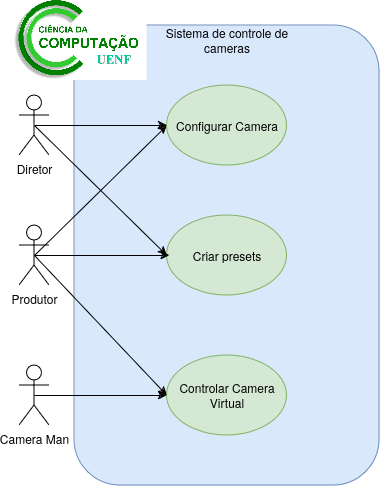
\includegraphics[width=0.8\textwidth]{Cameras}
    \caption{Diagrama de Sistema de cameras virtuais}
    \label{fig:diagram1}
\end{figure}

\subsection{Caso de Uso 2: Edição e Renderização de Vídeos}
\begin{description}[style=nextline]
    \item[Descrição:] Os editores utilizam este caso de uso para editar, ajustar efeitos visuais e renderizar vídeos usando os computadores de alta performance conectados ao servidor central. Os arquivos grandes são transmitidos diretamente do servidor para facilitar o trabalho.
    
    \item[Atores:] Editores de vídeo, Produtores.
    
    \item[Ações:]
    \begin{enumerate}
        \item Carregar os arquivos de vídeo e efeitos necessários.
        \item Realizar a edição, incluindo cortes, ajustes e aplicação de efeitos.
        \item Iniciar a renderização do vídeo.
        \item Enviar Feedback para os editores
    \end{enumerate}
\end{description}

\begin{figure}[ht]
    \centering
    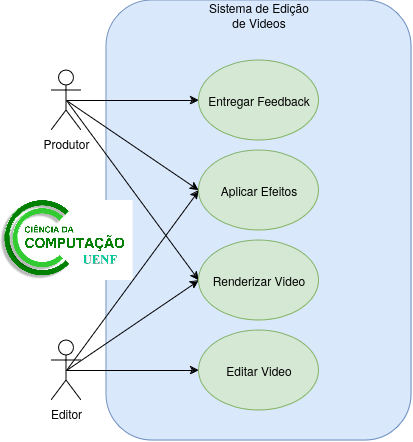
\includegraphics[width=0.8\textwidth]{Editores}
    \caption{Diagrama de Interação Editor Sistema}
    \label{fig:diagram1}
\end{figure}

\subsection{Caso de Uso 3: Gerenciamento de Projetos}
\begin{description}[style=nextline]
    \item[Descrição:] Este caso de uso permite o controle e acompanhamento de projetos no sistema. O cliente pode acessar um site interno para ver o progresso do projeto, dar feedback, e visualizar atualizações diretamente.
    
    \item[Atores:] Gerente de Projetos, Cliente.
    
    \item[Pré-condição:] O projeto está registrado no sistema com acesso disponível para o cliente.
    
    \item[Sequência de Ações:]
    \begin{enumerate}
        \item O gerente de projetos atualiza o status do projeto no sistema.
        \item O cliente acessa o site interno para verificar o andamento do projeto.
        \item O cliente visualiza o progresso, dá feedback e faz marcações se necessário.
        \item O gerente de projetos visualiza o feedback e atualiza o projeto conforme solicitado.
    \end{enumerate}
    
    \item[Pós-condição:] O projeto é atualizado de acordo com o feedback do cliente e segue para as próximas etapas.
\end{description}

\begin{figure}[ht]
    \centering
    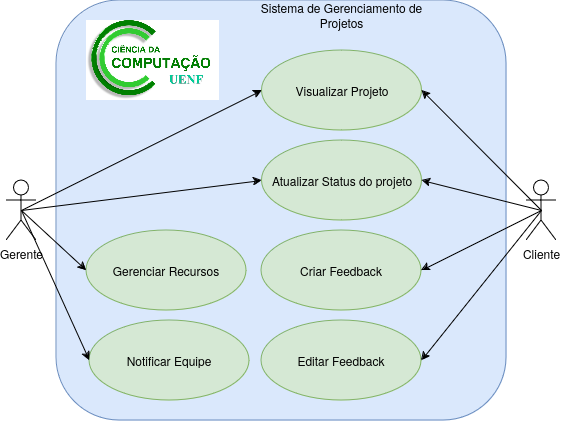
\includegraphics[width=0.8\textwidth]{Gerenciar}
    \caption{Diagrama de Interação Cliente/Gerente Sistema}
    \label{fig:diagram1}
\end{figure}

\pagebreak
\newpage

\section{Modelagem do Sistema}

Esta seção descreve a modelagem do sistema, incluindo a estruturação de dados e os processos principais. A modelagem de dados representa a estrutura e o armazenamento de informações, enquanto a modelagem de processos detalha o fluxo de dados e operações nos subsistemas principais.

\subsection{Modelagem de Processos: Subsistema Renderizacao de Cenas}
O subsistema de renderização lida com a aplicação de efeitos e o processamento das cenas. Ele transforma o trabalho dos esditores na cena final disponivel para os clientes.

\begin{itemize}
    \item \textbf{Dados de Entrada}: Arquivos de vídeo brutos, configurações de efeitos visuais.
    \item \textbf{Processos}:
        \begin{itemize}
            \item \textbf{Aplicar Efeitos}: O servidor aplica efeitos visuais, com as configurações configuradas pelos editores na edição.
            \item \textbf{Renderizacao de Video}: Após os efeitos, a cena é renderizada e salva no servidor.
        \end{itemize}
    \item \textbf{Dados de Saída}: Cena finalizada, pronta para visualização ou download.
\end{itemize}

\begin{figure}[ht]
    \centering
    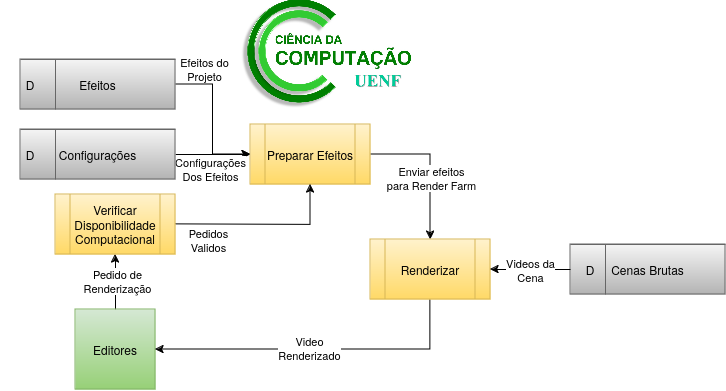
\includegraphics[width=0.8\textwidth]{Videos}
    \caption{Diagrama de Processo de Renderizacao}
    \label{fig:diagram1}
\end{figure}

\pagebreak
\newpage

\subsection{Modelagem de Processos: Subsistema de Gerenciamento de Feedback e Progresso}
O subsistema de gerenciamento de feedback e progresso armazena as atualizações de projetos e feedbacks dos clientes, permitindo o acompanhamento contínuo.

\begin{itemize}
    \item \textbf{Dados de Entrada}: Atualizações de status de projeto, feedbacks dos clientes.
    \item \textbf{Processos}:
        \begin{itemize}
            \item \textbf{Armazenamento de feedback}: Feedbacks sobre os vídeos são coletados e armazenados.
            \item \textbf{Atualização de Progresso do Projeto}: O status do projeto é atualizado e salvo no banco de dados.
        \end{itemize}
    \item \textbf{Dados de Saída}: Relatórios de progresso e feedbacks dos clientes.
\end{itemize}

\begin{figure}[ht]
    \centering
    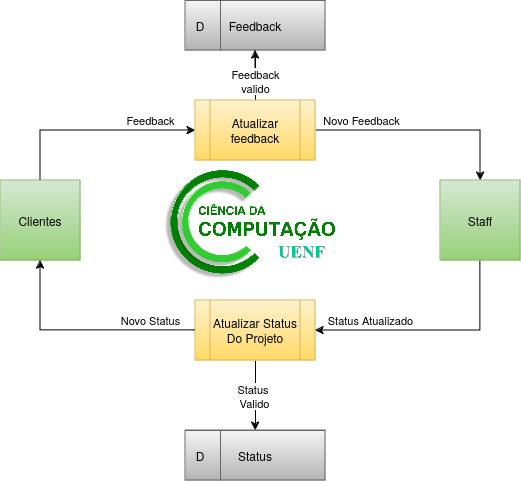
\includegraphics[width=0.8\textwidth]{Feedback}
    \caption{Diagrama de Processo de Feedbacks e Progresso}
    \label{fig:diagram1}
\end{figure}

\pagebreak
\newpage

\subsection{Modelagem de Processos: Subsistema de Gerenciamento de Recursos de Projeto}
Este subsistema gerencia os arquivos e recursos do projeto, organizando o tempo do time com base no que o cliente deseja pronto.

\begin{itemize}
    \item \textbf{Dados de Entrada}: metadados do projeto, pedidos do cliente
    \item \textbf{Processos}:
        \begin{itemize}
            \item \textbf{Planejamento de Recursos}: A alocação de recursos é calculada com base as necessidades do cliente
            \item \textbf{Atualização do projeto}: O projeto é atualizado no banco para ter as novas datas e demandas salvas
            \item \textbf{Notificação da Equipe}: A equipe é notificada de suas novas prioridades
        \end{itemize}
    \item \textbf{Dados de Saída}: Relatório de recursos do projeto atualizado
\end{itemize}

\begin{figure}[ht]
    \centering
    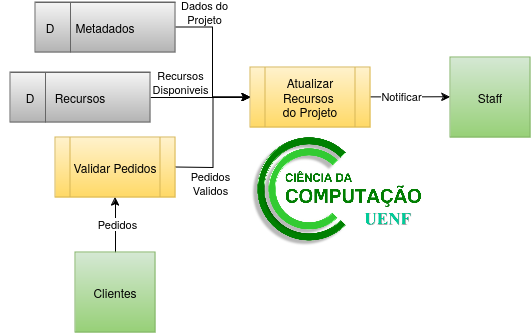
\includegraphics[width=0.8\textwidth]{Recursos}
    \caption{Diagrama de Processo de Recursos}
    \label{fig:diagram1}
\end{figure}

\pagebreak
\newpage

Nesta seção, detalhamos a modelagem de dados para os principais subsistemas do sistema de estúdio de filmagem e edição. Cada diagrama de Entidade-Relacionamento (DER) a seguir apresenta as entidades, atributos e os relacionamentos essenciais para a estrutura de dados do sistema.

\subsection{Modelagem de Dados DER-01: Central de Edição}
O primeiro diagrama modela o subsistema da Central de Edição, onde os editores manipulam arquivos de vídeo e utilizam software especializado para editar o conteúdo. As principais entidades deste modelo são:

\begin{itemize}
    \item \textbf{Central de Edição}: Representa o conjunto de estações de edição disponíveis no estúdio.
    \item \textbf{Estação de Edição}: Define cada estação individual, equipada com um computador e software.
    \item \textbf{Computador}: Contém informações sobre o hardware utilizado, como processador e memória RAM.
    \item \textbf{Software}: Inclui as ferramentas utilizadas para edição de vídeo e efeitos visuais.
    \item \textbf{Arquivo}: Representa os arquivos de vídeo e outros recursos manipulados durante a edição.
\end{itemize}

Este subsistema possui relacionamentos que indicam a utilização de computadores e software pelas estações de edição, bem como o acesso e manipulação de arquivos.

\begin{figure}[ht]
    \centering
    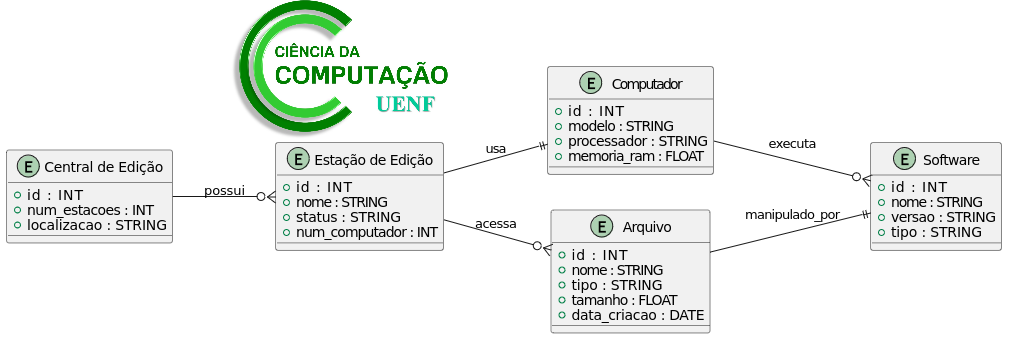
\includegraphics[width=0.8\textwidth]{EDICAO}
    \caption{Diagrama de Entidade-Relacionamento para a Central de Edição}
    \label{fig:edicao}
\end{figure}

\subsection{Modelagem de Dados DER-02: Centro de Filmagem}
O segundo diagrama modela o Centro de Filmagem, que é onde ocorre a captura das cenas utilizando câmeras virtuais e outros equipamentos. As entidades principais incluem:

\begin{itemize}
    \item \textbf{Centro de Filmagem}: Refere-se ao local onde são realizadas as gravações com a tela LED e equipamentos adicionais.
    \item \textbf{Câmera Virtual}: Utilizada para capturar a cena em conjunto com a tela infinita de LED.
    \item \textbf{Microfone}: Captura o áudio das cenas filmadas.
    \item \textbf{Tela LED (LED Screen)}: Uma tela utilizada para criar o cenário virtual.
    \item \textbf{Gravação}: Contém as informações sobre a filmagem realizada, incluindo o arquivo de saída.
    \item \textbf{Cenário Virtual}: Representa o ambiente digital usado nas gravações.
\end{itemize}

Os relacionamentos incluem a utilização de câmeras e microfones pelo centro de filmagem, bem como a captura e armazenamento das gravações realizadas.

\begin{figure}[ht]
    \centering
    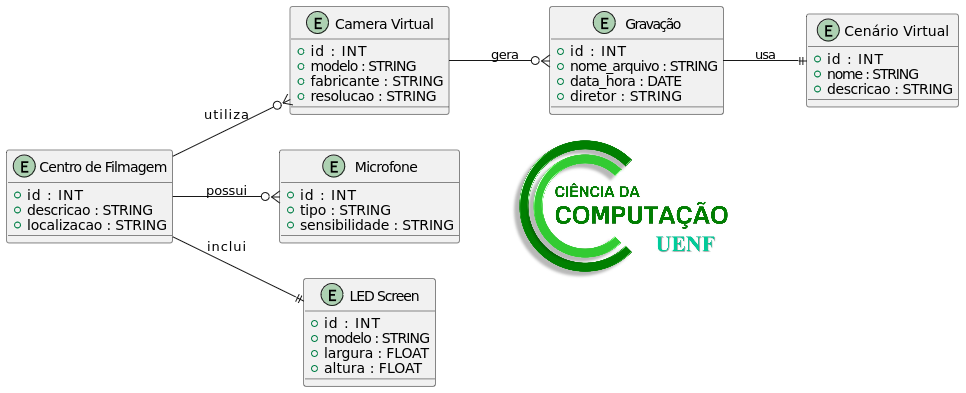
\includegraphics[width=0.8\textwidth]{FILMAGEM}
    \caption{Diagrama de Entidade-Relacionamento para o Centro de Filmagem}
    \label{fig:filmagem}
\end{figure}

\subsection{Modelagem de Dados DER-03: Centro de Motion Capture}
O terceiro diagrama apresenta o modelo de dados do Centro de Motion Capture, que é responsável pela captura de movimento usando trajes e câmeras especiais. As entidades principais são:

\begin{itemize}
    \item \textbf{Centro de Motion Capture}: Representa o local onde ocorre a captura de movimento.
    \item \textbf{Rokoko Suit}: Os trajes utilizados pelos atores para capturar movimentos detalhados.
    \item \textbf{Base Camera}: Câmeras instaladas para capturar os dados de movimento.
    \item \textbf{Computador Principal}: Processa os dados de tracking em tempo real.
    \item \textbf{Dados de Tracking}: Contém as informações capturadas durante o motion capture.
    \item \textbf{Ator}: Participa da captura vestindo o traje Rokoko.
\end{itemize}

\begin{figure}[ht]
    \centering
    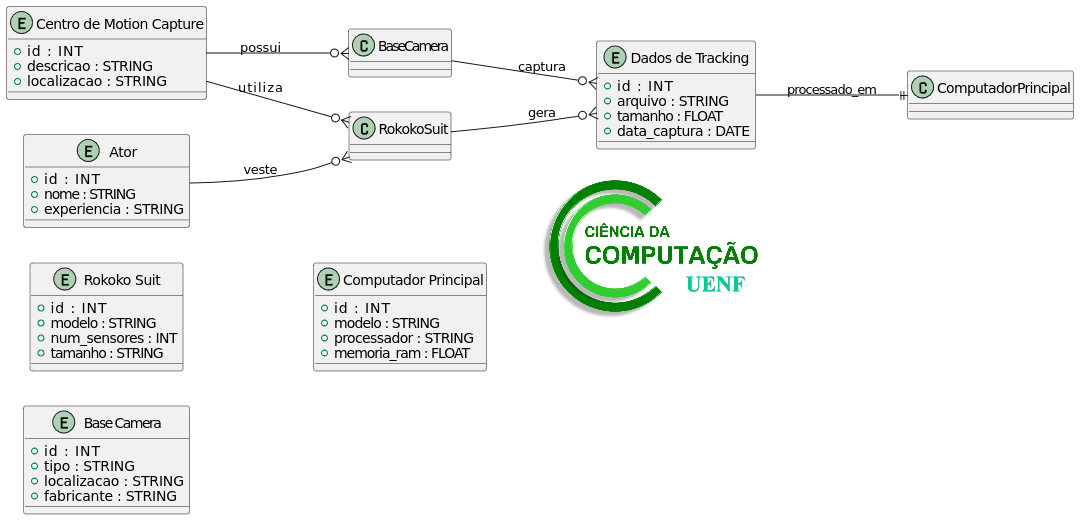
\includegraphics[width=0.8\textwidth]{MOTION}
    \caption{Diagrama de Entidade-Relacionamento para o Centro de Motion Capture}
    \label{fig:motion}
\end{figure}

O modelo inclui relacionamentos que indicam o uso dos trajes e câmeras pelo centro, e a geração e processamento dos dados de tracking pelos computadores.

\subsection{Modelagem de Dados DER-04: Centro de Scanning e Data Center}
O quarto diagrama apresenta o modelo de dados para o Centro de Scanning e o Data Center, que lida com a digitalização 3D e o armazenamento dos dados escaneados. As principais entidades são:

\begin{itemize}
    \item \textbf{Centro de Scanning}: Local onde são realizados os scans 3D de objetos e pessoas.
    \item \textbf{Camera LIDAR}: Equipamento utilizado para capturar imagens e dados 3D.
    \item \textbf{Scan 3D}: Armazena os arquivos resultantes das digitalizações.
    \item \textbf{Objeto Escaneado}: Representa o sujeito da digitalização 3D.
    \item \textbf{Data Center}: Armazena os arquivos de scan e realiza backups.
    \item \textbf{Backup}: Contém as informações de backup dos dados escaneados.
\end{itemize}

Os relacionamentos incluem a captura de dados pelas câmeras LIDAR e o armazenamento dos scans no Data Center, com backups realizados periodicamente.

\begin{figure}[ht]
    \centering
    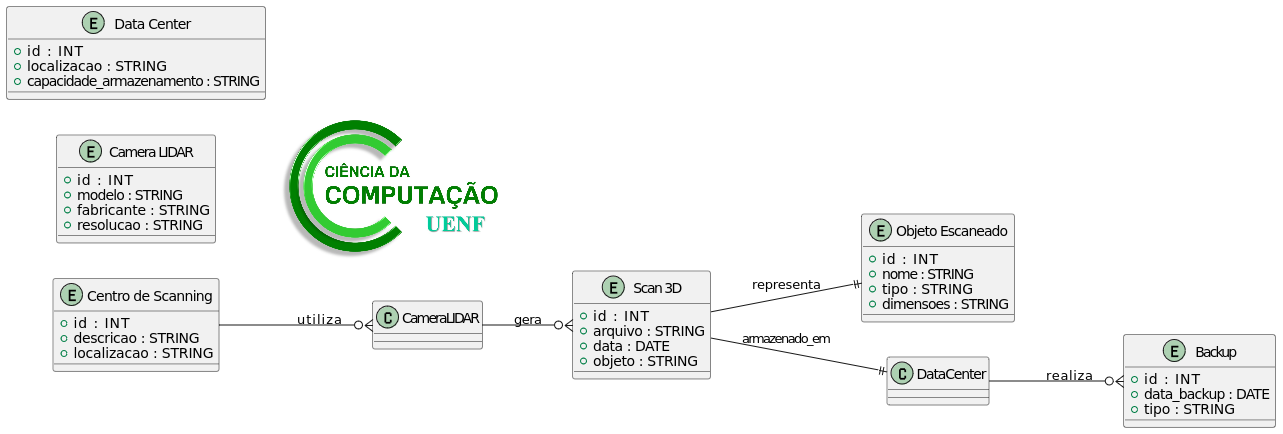
\includegraphics[width=0.8\textwidth]{DATA}
    \caption{Diagrama de Entidade-Relacionamento para o Centro de Scanning e Data Center}
    \label{fig:data}
\end{figure}

\subsection{Modelagem de Dados DER-05: Servidor Interno e Website}
O quinto diagrama modela a estrutura de dados para o Servidor Interno e o Website, que são responsáveis pelo armazenamento de arquivos de projeto e interação com os clientes. As entidades são:

\begin{itemize}
    \item \textbf{Servidor Interno}: Centraliza o armazenamento dos arquivos e gerencia as conexões internas.
    \item \textbf{Arquivo de Projeto}: Representa os arquivos associados aos projetos, incluindo vídeos e documentos.
    \item \textbf{Usuário Cliente}: Contém informações sobre os clientes que acessam o sistema.
    \item \textbf{Feedback}: Armazena os comentários e sugestões dos clientes sobre os projetos.
    \item \textbf{Website}: Interface pública que permite aos clientes visualizar e fornecer feedback sobre os projetos.
\end{itemize}

Os relacionamentos deste modelo incluem o armazenamento de arquivos pelo servidor, o envio de feedback pelos clientes e a integração com o website para coleta de comentários e relatórios de progresso.

\begin{figure}[ht]
    \centering
    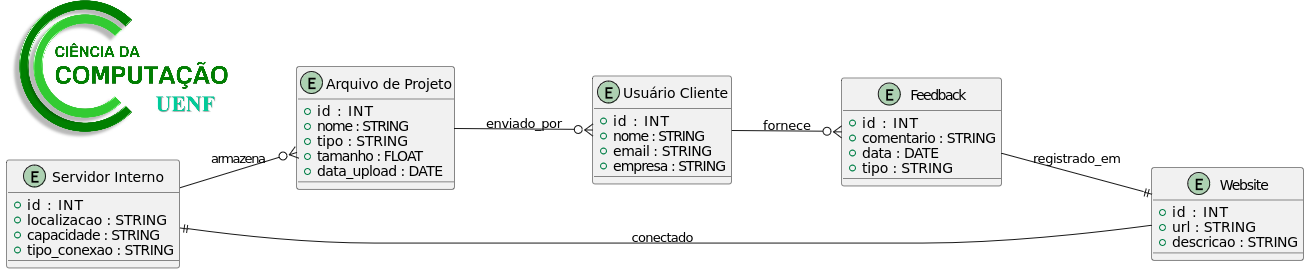
\includegraphics[width=0.8\textwidth]{SERVIDOR}
    \caption{Diagrama de Entidade-Relacionamento para o Servidor Interno e Website}
    \label{fig:servidor}
\end{figure}

